% Options for packages loaded elsewhere
\PassOptionsToPackage{unicode}{hyperref}
\PassOptionsToPackage{hyphens}{url}
%
\documentclass[
]{article}
\title{Data Analysis including 2020 and 2021 Season.''Development of
criteria for variable N-fertilizer and irrigation management of
potatoes''}
\author{Fernando Bortolozo}
\date{10/29/2021}

\usepackage{amsmath,amssymb}
\usepackage{lmodern}
\usepackage{iftex}
\ifPDFTeX
  \usepackage[T1]{fontenc}
  \usepackage[utf8]{inputenc}
  \usepackage{textcomp} % provide euro and other symbols
\else % if luatex or xetex
  \usepackage{unicode-math}
  \defaultfontfeatures{Scale=MatchLowercase}
  \defaultfontfeatures[\rmfamily]{Ligatures=TeX,Scale=1}
\fi
% Use upquote if available, for straight quotes in verbatim environments
\IfFileExists{upquote.sty}{\usepackage{upquote}}{}
\IfFileExists{microtype.sty}{% use microtype if available
  \usepackage[]{microtype}
  \UseMicrotypeSet[protrusion]{basicmath} % disable protrusion for tt fonts
}{}
\makeatletter
\@ifundefined{KOMAClassName}{% if non-KOMA class
  \IfFileExists{parskip.sty}{%
    \usepackage{parskip}
  }{% else
    \setlength{\parindent}{0pt}
    \setlength{\parskip}{6pt plus 2pt minus 1pt}}
}{% if KOMA class
  \KOMAoptions{parskip=half}}
\makeatother
\usepackage{xcolor}
\IfFileExists{xurl.sty}{\usepackage{xurl}}{} % add URL line breaks if available
\IfFileExists{bookmark.sty}{\usepackage{bookmark}}{\usepackage{hyperref}}
\hypersetup{
  pdftitle={Data Analysis including 2020 and 2021 Season.''Development of criteria for variable N-fertilizer and irrigation management of potatoes''},
  pdfauthor={Fernando Bortolozo},
  hidelinks,
  pdfcreator={LaTeX via pandoc}}
\urlstyle{same} % disable monospaced font for URLs
\usepackage[margin=1in]{geometry}
\usepackage{graphicx}
\makeatletter
\def\maxwidth{\ifdim\Gin@nat@width>\linewidth\linewidth\else\Gin@nat@width\fi}
\def\maxheight{\ifdim\Gin@nat@height>\textheight\textheight\else\Gin@nat@height\fi}
\makeatother
% Scale images if necessary, so that they will not overflow the page
% margins by default, and it is still possible to overwrite the defaults
% using explicit options in \includegraphics[width, height, ...]{}
\setkeys{Gin}{width=\maxwidth,height=\maxheight,keepaspectratio}
% Set default figure placement to htbp
\makeatletter
\def\fps@figure{htbp}
\makeatother
\setlength{\emergencystretch}{3em} % prevent overfull lines
\providecommand{\tightlist}{%
  \setlength{\itemsep}{0pt}\setlength{\parskip}{0pt}}
\setcounter{secnumdepth}{-\maxdimen} % remove section numbering
\usepackage{booktabs}
\usepackage{longtable}
\usepackage{array}
\usepackage{multirow}
\usepackage{wrapfig}
\usepackage{float}
\usepackage{colortbl}
\usepackage{pdflscape}
\usepackage{tabu}
\usepackage{threeparttable}
\usepackage{threeparttablex}
\usepackage[normalem]{ulem}
\usepackage{makecell}
\usepackage{xcolor}
\ifLuaTeX
  \usepackage{selnolig}  % disable illegal ligatures
\fi

\begin{document}
\maketitle

\hypertarget{exploratory-analisys}{%
\section{1. Exploratory Analisys}\label{exploratory-analisys}}

Total yield distribution across sites,irrigation methods and season for
In-season decision, Grower's practice and UF/IFAS N-fertilizer
application. The total yield response was 28687.47, 29676.20, and
29411.81 lbs./acre for fixed N application rate, grower's practice, and
in-season decision N application respectively. There is no significant
statistical difference between treatments. This results did not specify
factor such as site, irrigation and year.

\hypertarget{summary}{%
\subsection{\texorpdfstring{\textbf{1.1
Summary}}{1.1 Summary}}\label{summary}}

\begin{verbatim}
##      Trt                Trt_              n_rates      date              dap   
##  Length:84          Length:84          Min.   :0.0   Mode:logical   Min.   :0  
##  Class :character   Class :character   1st Qu.:0.0   NA's:84        1st Qu.:0  
##  Mode  :character   Mode  :character   Median :0.5                  Median :0  
##                                        Mean   :1.0                  Mean   :0  
##                                        3rd Qu.:2.0                  3rd Qu.:0  
##                                        Max.   :3.0                  Max.   :0  
##       time           farm              irrig                year     
##  Min.   :5.000   Length:84          Length:84          Min.   :2020  
##  1st Qu.:5.000   Class :character   Class :character   1st Qu.:2020  
##  Median :5.000   Mode  :character   Mode  :character   Median :2020  
##  Mean   :5.429                                         Mean   :2020  
##  3rd Qu.:6.000                                         3rd Qu.:2021  
##  Max.   :6.000                                         Max.   :2021  
##       plot            block           tyield     
##  Min.   : 1.000   Min.   :1.000   Min.   : 1568  
##  1st Qu.: 3.000   1st Qu.:1.000   1st Qu.:28570  
##  Median : 6.000   Median :2.000   Median :31491  
##  Mean   : 5.857   Mean   :2.286   Mean   :29258  
##  3rd Qu.: 8.000   3rd Qu.:3.000   3rd Qu.:34492  
##  Max.   :12.000   Max.   :4.000   Max.   :50730
\end{verbatim}

\begin{verbatim}
## 
##  Shapiro-Wilk normality test
## 
## data:  dados$tyield
## W = 0.73811, p-value = 6.148e-11
\end{verbatim}

\hypertarget{total-yield-for-sseepage-sep-and-subirrigation-drain-tile-sdt}{%
\section{1.2. Total yield for Sseepage (SEP) and Subirrigation Drain
Tile
(SDT)}\label{total-yield-for-sseepage-sep-and-subirrigation-drain-tile-sdt}}

\hypertarget{figure-1.total-yield-response-considering-n-rates-fertilizer-for-arlie-and-parker-accounting-2020-and-2021-season-for-seepage-sep-irr.-system.}{%
\paragraph{\texorpdfstring{\textbf{Figure 1.}Total Yield Response
considering N rates Fertilizer for Arlie and Parker accounting 2020 and
2021 Season for Seepage (SEP) Irr.
System.}{Figure 1.Total Yield Response considering N rates Fertilizer for Arlie and Parker accounting 2020 and 2021 Season for Seepage (SEP) Irr. System.}}\label{figure-1.total-yield-response-considering-n-rates-fertilizer-for-arlie-and-parker-accounting-2020-and-2021-season-for-seepage-sep-irr.-system.}}

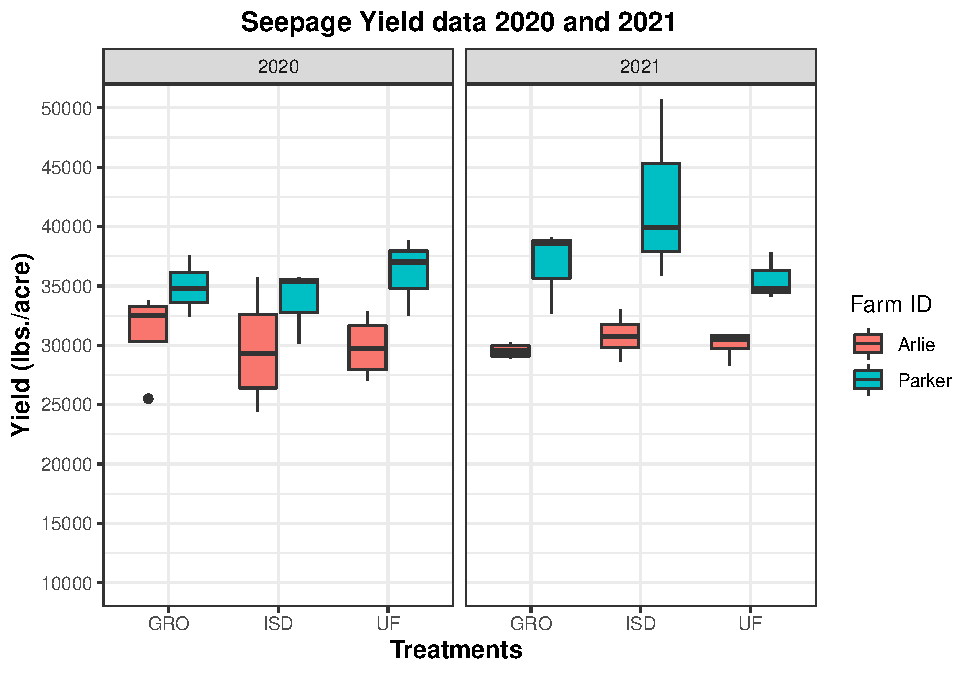
\includegraphics{NoffsiteT_files/figure-latex/unnamed-chunk-2-1.pdf}
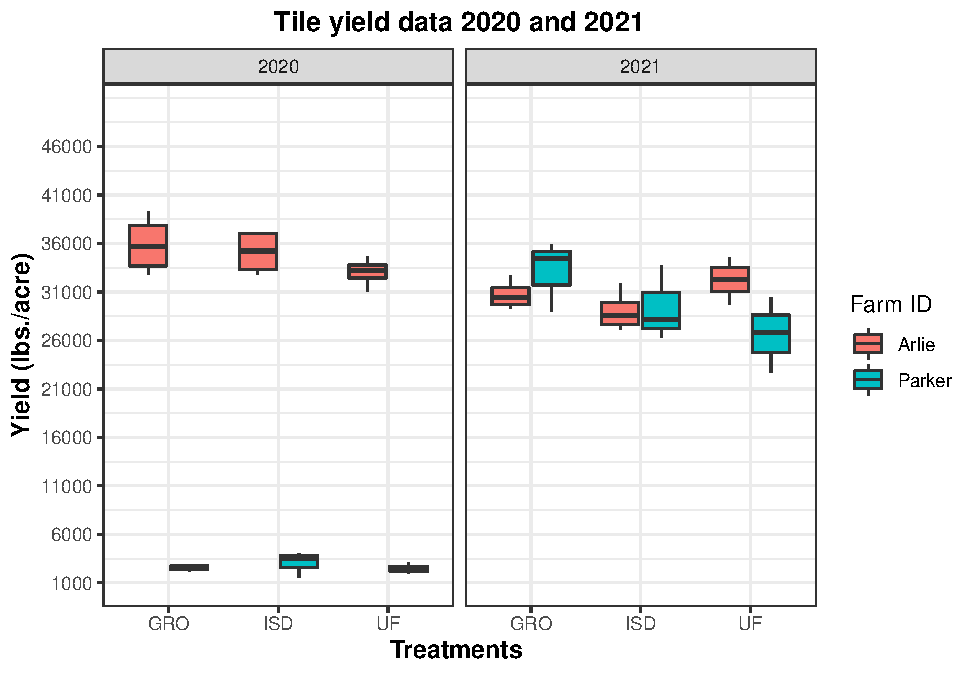
\includegraphics{NoffsiteT_files/figure-latex/unnamed-chunk-2-2.pdf}

\hypertarget{anova-and-tukeyhsd-test}{%
\subsubsection{\texorpdfstring{\textbf{Anova and TukeyHSD
test}}{Anova and TukeyHSD test}}\label{anova-and-tukeyhsd-test}}

\hypertarget{figure-2.-total-yield-distribution-across-farms-irr.-systems-and-year-for-each-treatment}{%
\paragraph{\texorpdfstring{\textbf{Figure 2.} Total Yield distribution
Across Farms, Irr. Systems, and Year for Each
Treatment}{Figure 2. Total Yield distribution Across Farms, Irr. Systems, and Year for Each Treatment}}\label{figure-2.-total-yield-distribution-across-farms-irr.-systems-and-year-for-each-treatment}}

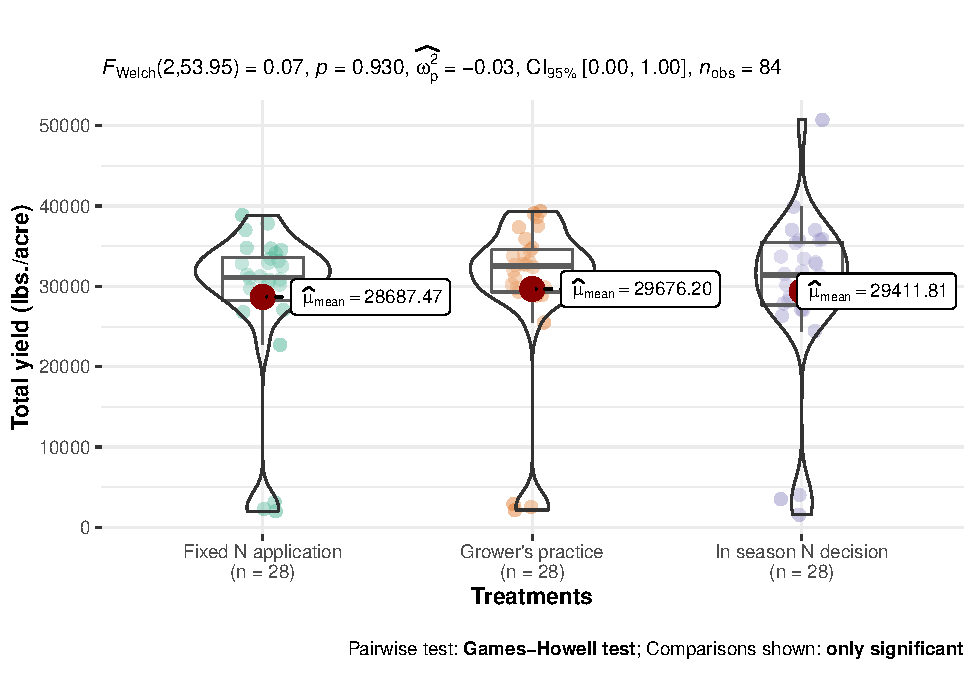
\includegraphics{NoffsiteT_files/figure-latex/unnamed-chunk-3-1.pdf}

\hypertarget{pairwise-test}{%
\subsubsection{\texorpdfstring{\textbf{Pairwise
test}}{Pairwise test}}\label{pairwise-test}}

\hypertarget{figure-2.-total-yield-distribution-across-farms-irr.-systems-and-year-for-each-treatment-1}{%
\paragraph{\texorpdfstring{\textbf{Figure 2.} Total Yield distribution
Across Farms, Irr. Systems, and Year for Each
Treatment}{Figure 2. Total Yield distribution Across Farms, Irr. Systems, and Year for Each Treatment}}\label{figure-2.-total-yield-distribution-across-farms-irr.-systems-and-year-for-each-treatment-1}}

\begin{verbatim}
##             Df    Sum Sq   Mean Sq F value Pr(>F)
## Trt          2 1.467e+07   7336787    0.07  0.932
## Residuals   81 8.467e+09 104531808
\end{verbatim}

\begin{verbatim}
##   Tukey multiple comparisons of means
##     95% family-wise confidence level
## 
## Fit: aov(formula = tyield ~ Trt, data = dados)
## 
## $Trt
##                                               diff       lwr      upr     p adj
## Grower's practice-Fixed N application     988.7342 -5535.239 7512.707 0.9304371
## In season N decision-Fixed N application  724.3406 -5799.633 7248.314 0.9620229
## In season N decision-Grower's practice   -264.3936 -6788.367 6259.580 0.9948520
\end{verbatim}

\begin{verbatim}
## $Trt
## $Trt$Letters
##    Grower's practice In season N decision  Fixed N application 
##                  "a"                  "a"                  "a" 
## 
## $Trt$LetterMatrix
##                         a
## Grower's practice    TRUE
## In season N decision TRUE
## Fixed N application  TRUE
\end{verbatim}

\begin{verbatim}
## # A tibble: 3 x 4
##   Trt                    mean  quant cld  
##   <chr>                 <dbl>  <dbl> <chr>
## 1 Grower's practice    29676. 34552. a    
## 2 In season N decision 29412. 35476. a    
## 3 Fixed N application  28687. 33642. a
\end{verbatim}

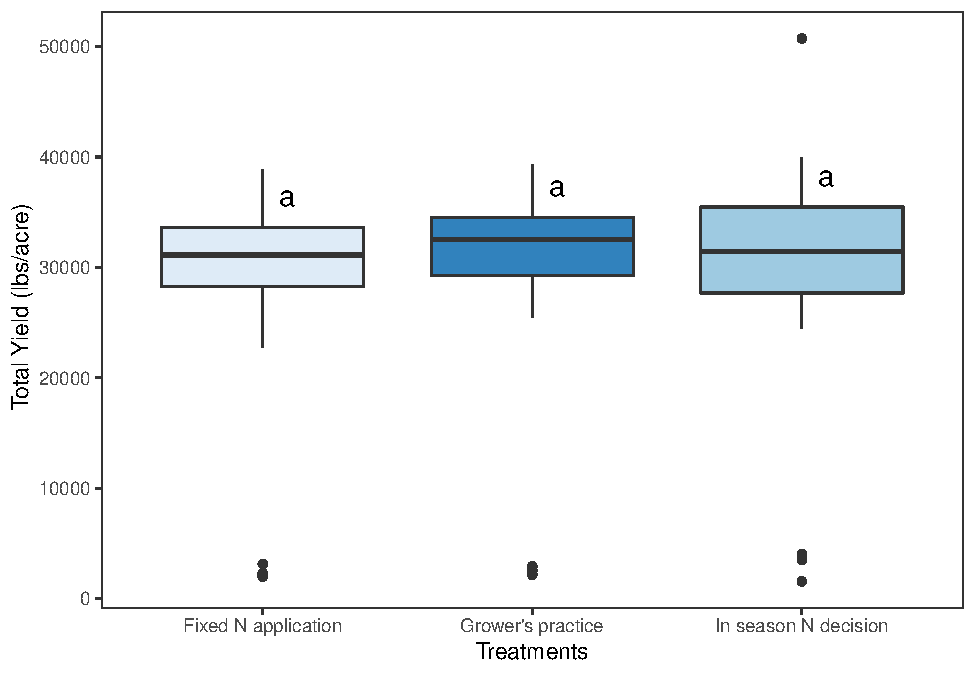
\includegraphics{NoffsiteT_files/figure-latex/unnamed-chunk-4-1.pdf}

\begin{enumerate}
\def\labelenumi{\arabic{enumi}.}
\setcounter{enumi}{2}
\tightlist
\item
  Total yield
\end{enumerate}

\hypertarget{figure-3.total-yield-response-considering-n-rates-fertilizer-for-arlie-and-parker-accounting-2020-and-2021-season-for-tile-sdt-irr.-system.}{%
\paragraph{\texorpdfstring{\textbf{Figure 3.}Total Yield Response
considering N rates Fertilizer for Arlie and Parker accounting 2020 and
2021 Season for Tile (SDT) Irr.
System.}{Figure 3.Total Yield Response considering N rates Fertilizer for Arlie and Parker accounting 2020 and 2021 Season for Tile (SDT) Irr. System.}}\label{figure-3.total-yield-response-considering-n-rates-fertilizer-for-arlie-and-parker-accounting-2020-and-2021-season-for-tile-sdt-irr.-system.}}

\hypertarget{total-yield-response-for-n-rates-for-sep-on-parker-at-2020}{%
\section{Total Yield Response for N rates for SEP on Parker at
2020}\label{total-yield-response-for-n-rates-for-sep-on-parker-at-2020}}

\begin{verbatim}
## ------------------------------------------------------------------------
## Analysis of Variance Table
## ------------------------------------------------------------------------
##            DF       SS       MS      Fc   Pr>Fc
## Treatament  2  8379822  4189911 0.67523 0.55890
## Block       2 29144357 14572179 2.34841 0.21154
## Residuals   4 24820482  6205121                
## Total       8 62344662                         
## ------------------------------------------------------------------------
## CV = 7.13 %
## 
## ------------------------------------------------------------------------
## Shapiro-Wilk normality test
## p-value:  0.7021718 
## According to Shapiro-Wilk normality test at 5% of significance, residuals can be considered normal.
## ------------------------------------------------------------------------
## 
## ------------------------------------------------------------------------
## Homogeneity of variances test
## p-value:  0.1434011 
## According to the test of oneillmathews at 5% of significance, the variances can be considered homocedastic.
## ------------------------------------------------------------------------
## 
## According to the F test, the means can not be considered distinct.
##   Levels    Means
## 1    GRO 34911.16
## 2    ISD 33769.89
## 3     UF 36133.02
## ------------------------------------------------------------------------
\end{verbatim}

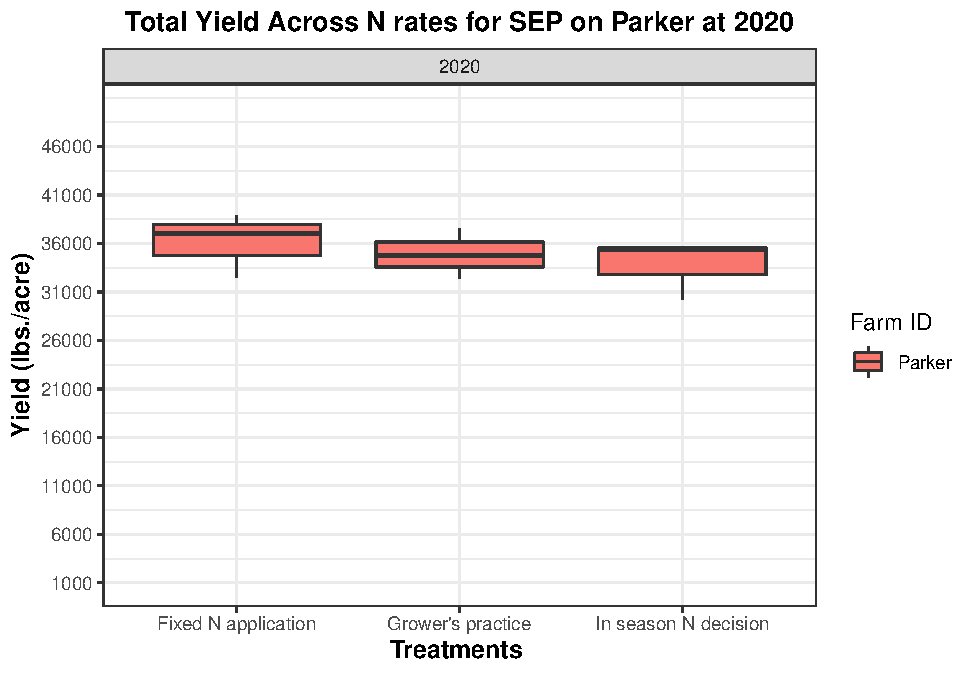
\includegraphics{NoffsiteT_files/figure-latex/unnamed-chunk-6-1.pdf}
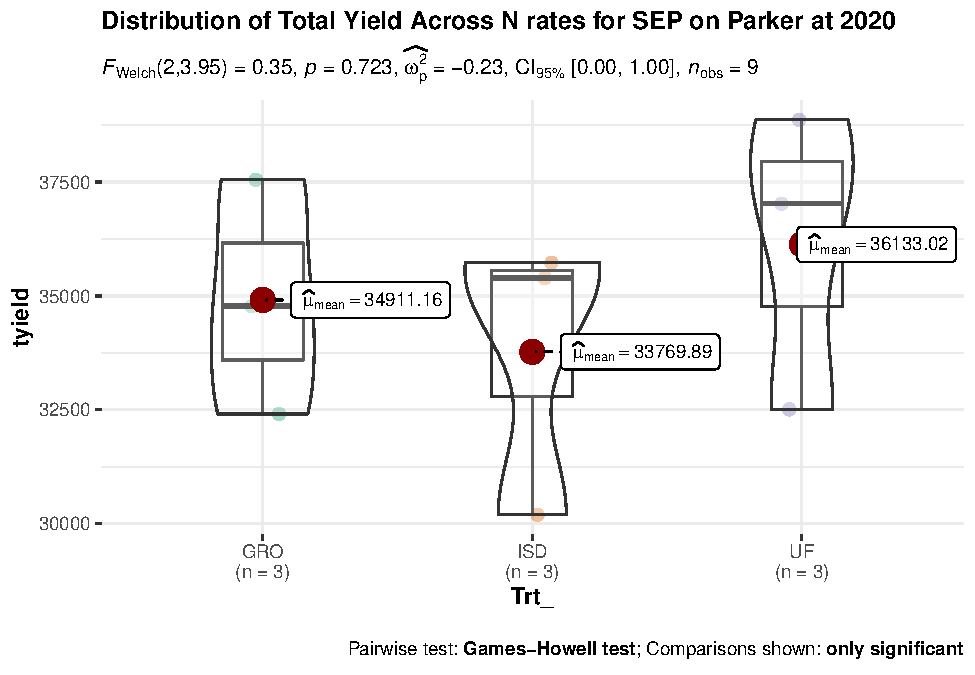
\includegraphics{NoffsiteT_files/figure-latex/unnamed-chunk-6-2.pdf}

\hypertarget{total-yield-response-for-n-rates-for-sep-on-parker-at-2021}{%
\section{Total Yield Response for N rates for SEP on Parker at
2021}\label{total-yield-response-for-n-rates-for-sep-on-parker-at-2021}}

\begin{verbatim}
## ------------------------------------------------------------------------
## Analysis of Variance Table
## ------------------------------------------------------------------------
##            DF        SS       MS     Fc   Pr>Fc
## Treatament  2  73787475 36893738 1.8691 0.26720
## Block       2  72245653 36122826 1.8301 0.27268
## Residuals   4  78954173 19738543               
## Total       8 224987301                        
## ------------------------------------------------------------------------
## CV = 11.63 %
## 
## ------------------------------------------------------------------------
## Shapiro-Wilk normality test
## p-value:  0.9753152 
## According to Shapiro-Wilk normality test at 5% of significance, residuals can be considered normal.
## ------------------------------------------------------------------------
## 
## ------------------------------------------------------------------------
## Homogeneity of variances test
## p-value:  0.1255436 
## According to the test of oneillmathews at 5% of significance, the variances can be considered homocedastic.
## ------------------------------------------------------------------------
## 
## According to the F test, the means can not be considered distinct.
##   Levels    Means
## 1    GRO 36795.68
## 2    ISD 42173.70
## 3     UF 35585.80
## ------------------------------------------------------------------------
\end{verbatim}

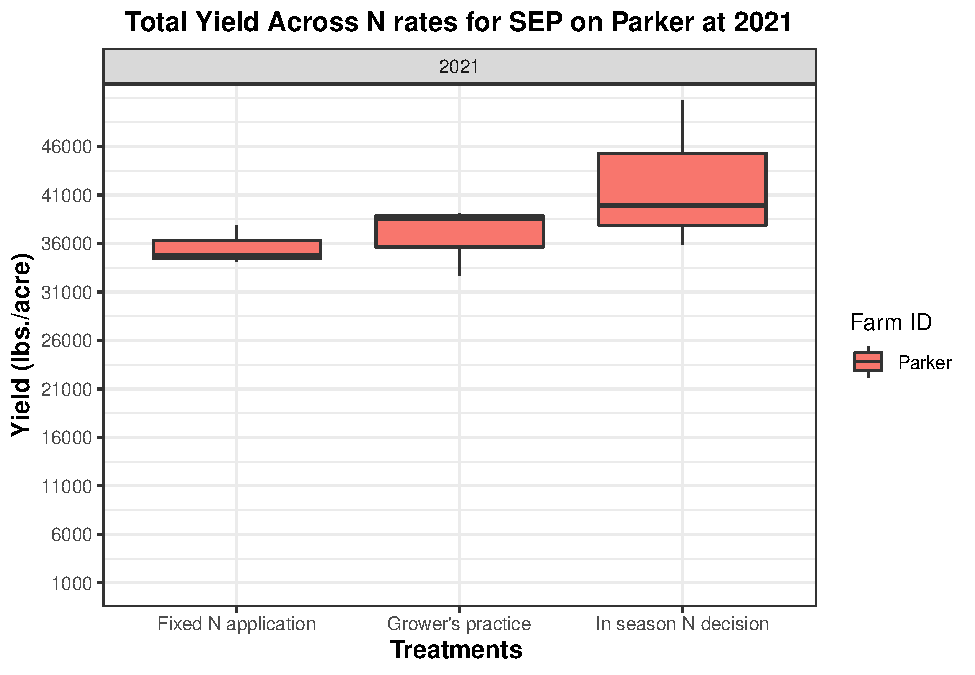
\includegraphics{NoffsiteT_files/figure-latex/unnamed-chunk-7-1.pdf}
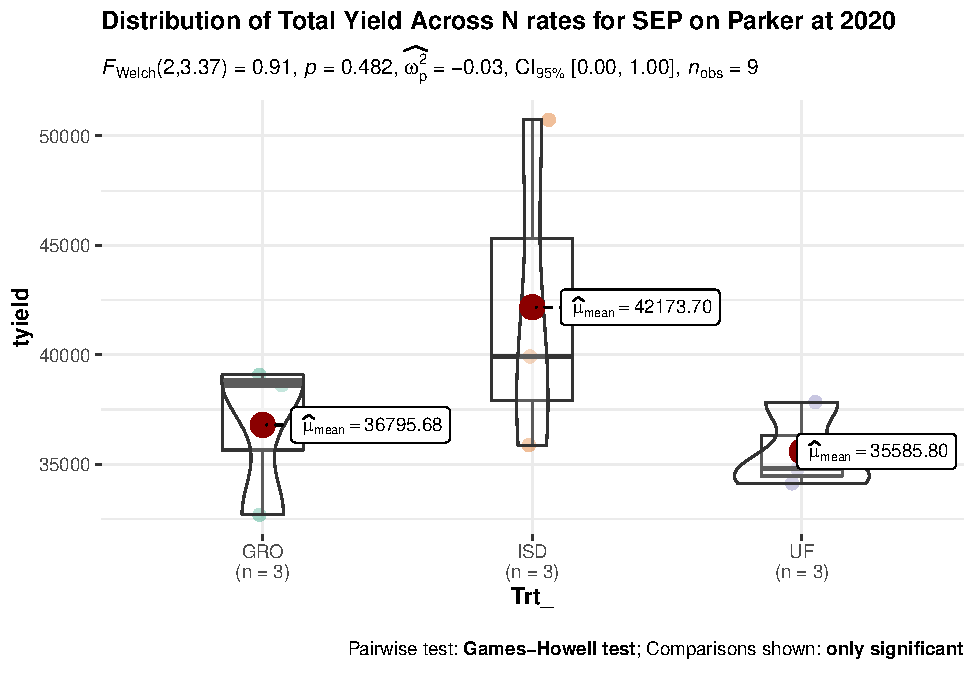
\includegraphics{NoffsiteT_files/figure-latex/unnamed-chunk-7-2.pdf}

\hypertarget{total-yield-response-for-n-rates-for-sep-on-smith-at-2020}{%
\section{Total Yield Response for N rates for SEP on Smith at
2020}\label{total-yield-response-for-n-rates-for-sep-on-smith-at-2020}}

\begin{verbatim}
## tibble [84 x 12] (S3: tbl_df/tbl/data.frame)
##  $ Trt    : chr [1:84] "Fixed N application" "Grower's practice" "In season N decision" "Grower's practice" ...
##  $ Trt_   : chr [1:84] "UF" "GRO" "ISD" "GRO" ...
##  $ n_rates: num [1:84] 3 1 2 1 3 2 3 1 2 3 ...
##  $ date   : logi [1:84] NA NA NA NA NA NA ...
##  $ dap    : num [1:84] 0 0 0 0 0 0 0 0 0 0 ...
##  $ time   : num [1:84] 5 5 5 5 5 5 5 5 5 5 ...
##  $ farm   : chr [1:84] "Arlie" "Arlie" "Arlie" "Arlie" ...
##  $ irrig  : chr [1:84] "SEEP" "SEEP" "SEEP" "SEEP" ...
##  $ year   : num [1:84] 2020 2020 2020 2020 2020 2020 2020 2020 2020 2020 ...
##  $ plot   : num [1:84] 1 2 3 4 5 6 7 8 9 10 ...
##  $ block  : num [1:84] 1 1 1 2 2 2 3 3 3 4 ...
##  $ tyield : num [1:84] 28233 33082 24444 25509 31239 ...
\end{verbatim}

\begin{verbatim}
## ------------------------------------------------------------------------
## Analysis of Variance Table
## ------------------------------------------------------------------------
##            DF        SS       MS      Fc   Pr>Fc
## Treatament  2   4563665  2281833 0.11718 0.89141
## Block       3  22141449  7380483 0.37903 0.77195
## Residuals   6 116832936 19472156                
## Total      11 143538051                         
## ------------------------------------------------------------------------
## CV = 14.61 %
## 
## ------------------------------------------------------------------------
## Shapiro-Wilk normality test
## p-value:  0.1251508 
## According to Shapiro-Wilk normality test at 5% of significance, residuals can be considered normal.
## ------------------------------------------------------------------------
## 
## ------------------------------------------------------------------------
## Homogeneity of variances test
## p-value:  0.8105969 
## According to the test of oneillmathews at 5% of significance, the variances can be considered homocedastic.
## ------------------------------------------------------------------------
## 
## According to the F test, the means can not be considered distinct.
##   Levels    Means
## 1    GRO 31078.97
## 2    ISD 29701.11
## 3     UF 29853.85
## ------------------------------------------------------------------------
\end{verbatim}

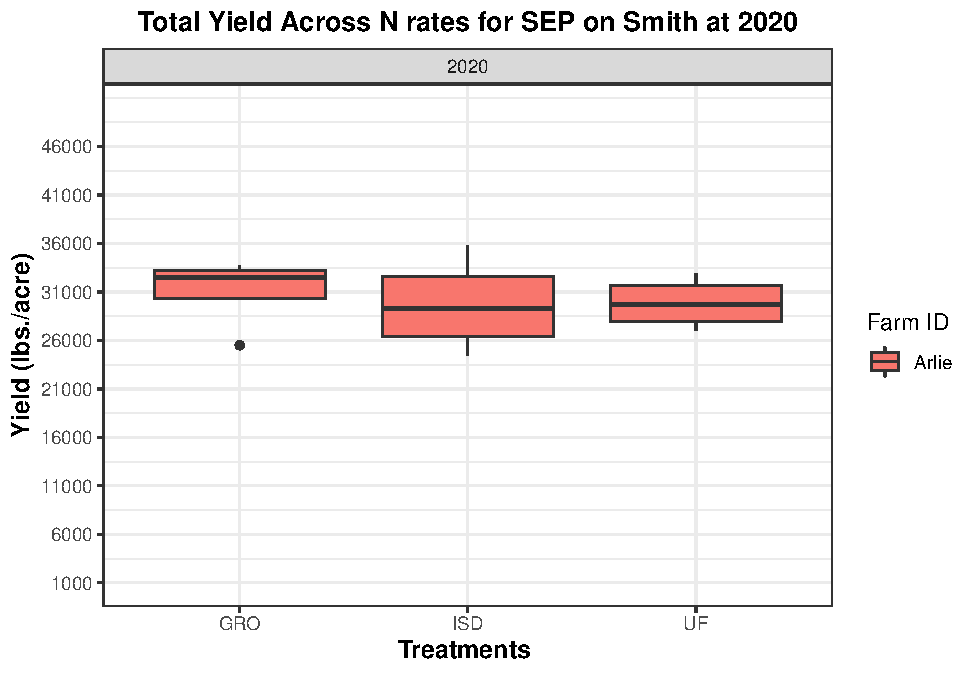
\includegraphics{NoffsiteT_files/figure-latex/unnamed-chunk-8-1.pdf}
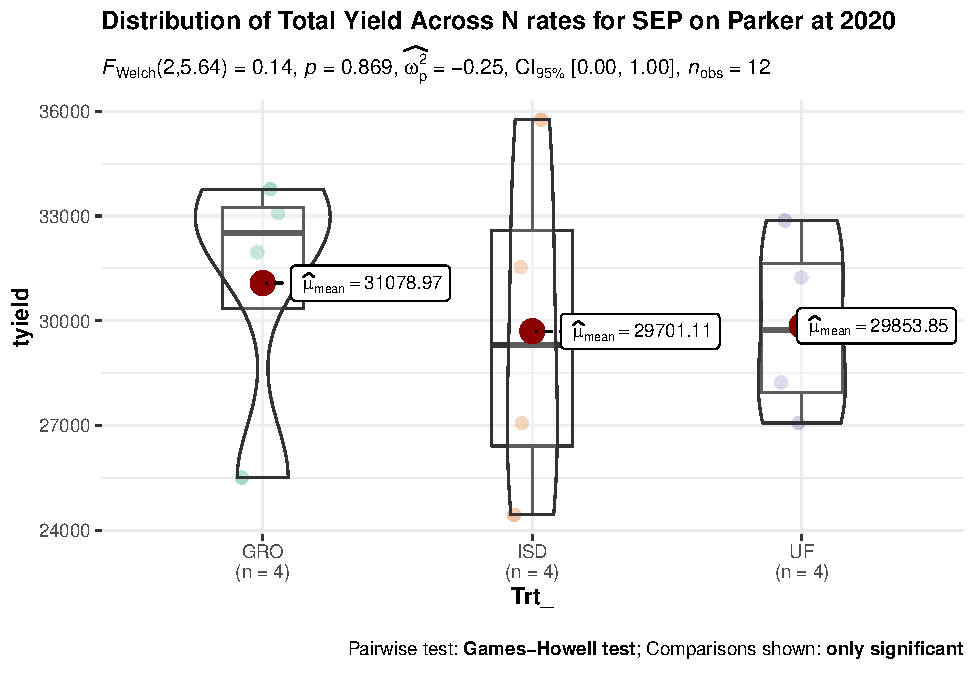
\includegraphics{NoffsiteT_files/figure-latex/unnamed-chunk-8-2.pdf}

\hypertarget{total-yield-response-for-n-rates-for-sep-on-smith-at-2021}{%
\section{Total Yield Response for N rates for SEP on Smith at
2021}\label{total-yield-response-for-n-rates-for-sep-on-smith-at-2021}}

\begin{verbatim}
## ------------------------------------------------------------------------
## Analysis of Variance Table
## ------------------------------------------------------------------------
##            DF        SS       MS      Fc   Pr>Fc
## Treatament  2   4563665  2281833 0.11718 0.89141
## Block       3  22141449  7380483 0.37903 0.77195
## Residuals   6 116832936 19472156                
## Total      11 143538051                         
## ------------------------------------------------------------------------
## CV = 14.61 %
## 
## ------------------------------------------------------------------------
## Shapiro-Wilk normality test
## p-value:  0.1251508 
## According to Shapiro-Wilk normality test at 5% of significance, residuals can be considered normal.
## ------------------------------------------------------------------------
## 
## ------------------------------------------------------------------------
## Homogeneity of variances test
## p-value:  0.8105969 
## According to the test of oneillmathews at 5% of significance, the variances can be considered homocedastic.
## ------------------------------------------------------------------------
## 
## According to the F test, the means can not be considered distinct.
##   Levels    Means
## 1    GRO 31078.97
## 2    ISD 29701.11
## 3     UF 29853.85
## ------------------------------------------------------------------------
\end{verbatim}

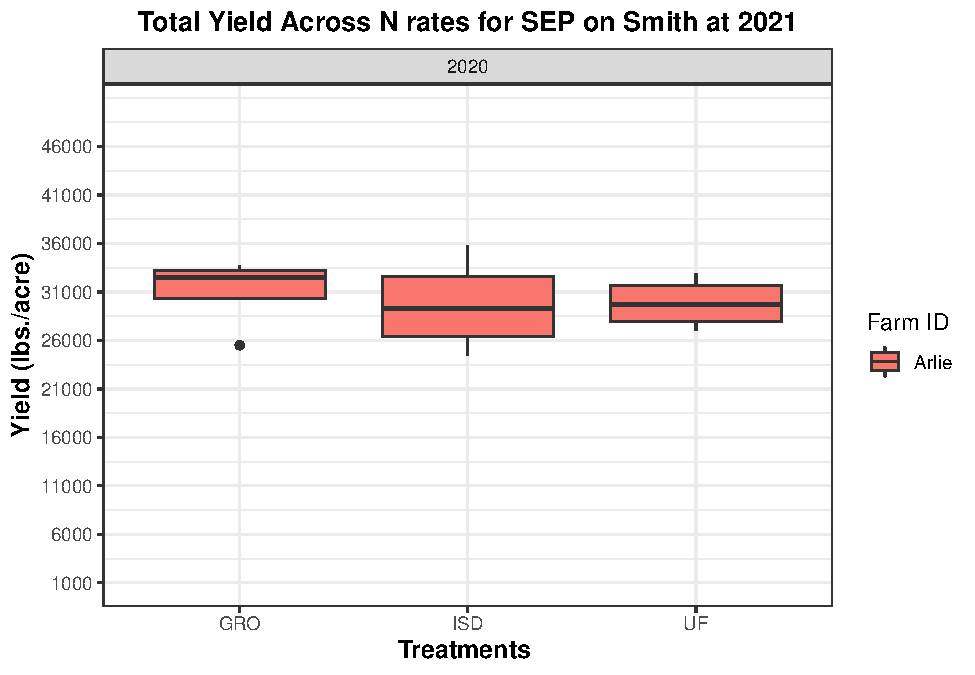
\includegraphics{NoffsiteT_files/figure-latex/unnamed-chunk-9-1.pdf}
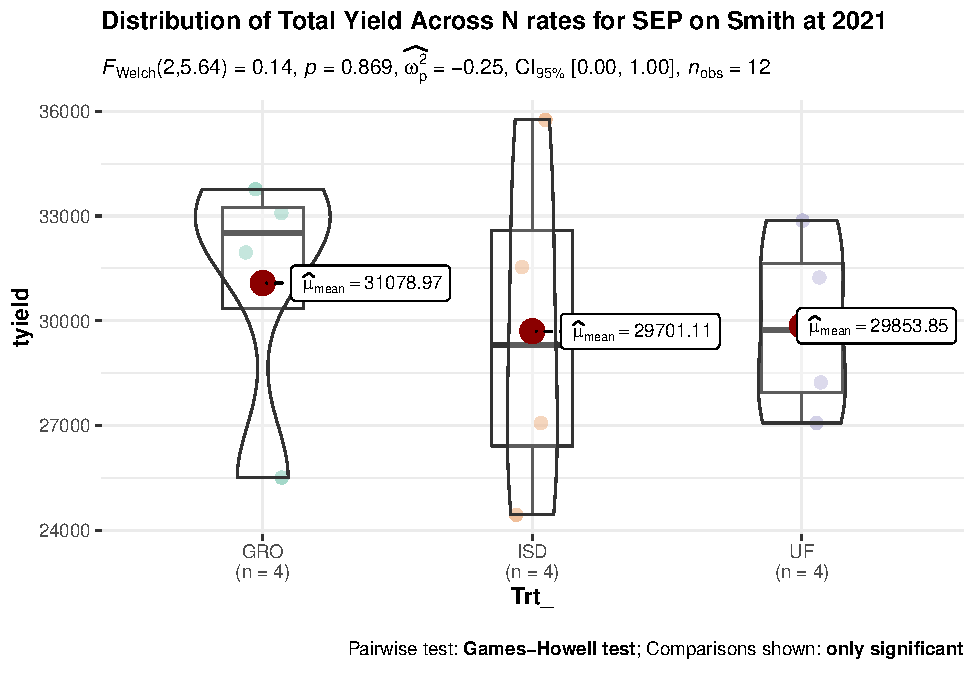
\includegraphics{NoffsiteT_files/figure-latex/unnamed-chunk-9-2.pdf}

\end{document}
